%----------------------------------------------------------------------------------------
%	PACKAGES AND DOCUMENT CONFIGURATIONS
%----------------------------------------------------------------------------------------

\documentclass{article}

\usepackage{graphicx}
\usepackage{listings}

%----------------------------------------------------------------------------------------
%	DOCUMENT INFORMATION
%----------------------------------------------------------------------------------------

\title{
	\begin{LARGE}
	\textbf{EE 445L - Lab 8: Software Drivers for an Embedded System\\Prep}
	\end{LARGE}
}

\author{Joshua Bryant \\ jmb6357 \and James Morris \\ jms3288}

\date{\today}

\begin{document}

\maketitle

\section{Schematic Design and Testing Differences}

	\begin{figure}[h]
		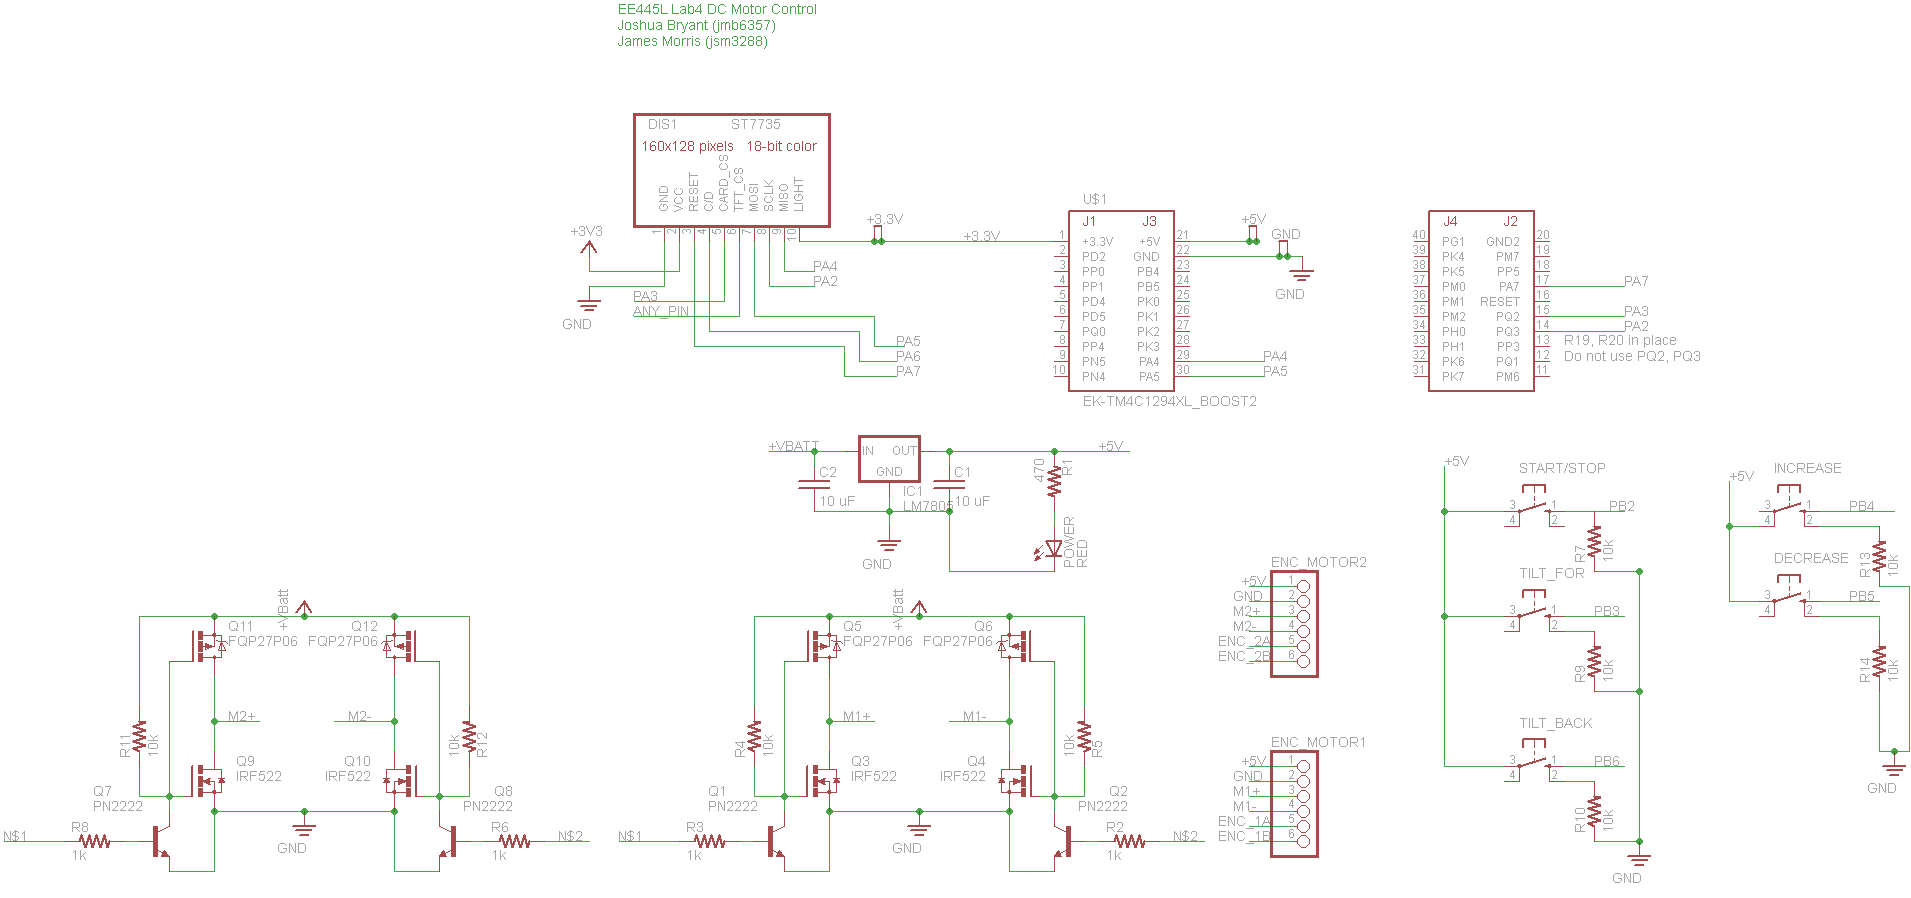
\includegraphics[keepaspectratio, width = \textwidth]{Lab8PrepGraphics/Ropebot_SchematicV2.png}
	\end{figure}
	
	The included schematic demonstrates both testing and intended final setup of the circuit. The only difference between the current version and the final board is that only headers for one set of breakout pins will be included on the board and the other pins needed will be reached via wires from the board to the appropriate header and pin locations on the board.\newpage

\section{Header Files}

The \textit{encoder.h} header file contains all the function definitions for interfacing with the quadrature encoders. The code currently only accepts quadrature encoders. This may change in the future depending on available time and motivation.
\lstinputlisting[language = C, frame = single]{encoder.h}

\par The \textit{motor.h} header file contains all the function definitions for interfacing with the brushed DC motors.
\lstinputlisting[language = C, frame = single]{motor.h}


\end{document}